%%%%%%%%%%%%%%%%%%%%%%%%%%%%%%%%%%%%%%%%%%%%%%%%%%%%%%%%%%%%%%%%%%%%
\chapter{Experimentos e Resultados}\label{experimentos}
Neste capítulo são apresentados os experimentos comparativos de estratégias
e seus resultados.
Na Seção \ref{prep}, é definido o subconjunto de estratégias e algoritmos de aprendizado
mais relevantes para os experimentos.
Nas demais seções é feita a demonstração de que as estratégias propostas SGmulti e
agnóstica baseada em densidade (prefixo ATU) são competitivas \ano{são mesmo?}.
Adicionalmente, constatações relevantes para o problema da escolha de estratégias
são fornecidas.
A análise experimental é dividida em duas partes: \ano{rever}
\textit{comparativa}, na Seção \ref{geral}, em que as estratégias são comparadas
entre si;
e, de \textit{recomendação automática},
na Seção \ref{isolado}.

\section{Preparação} \label{prep}
Devido à grande quantidade de fatores envolvidos nos experimentos,
faz-se necessária uma etapa de preparação em que apenas
a parcela mais representativa das estratégias e algoritmos de aprendizado
seja mantida.

\subsection{Diversidade dos algoritmos de aprendizado}\label{algs}
Uma forma indireta de ilustrar a diversidade entre os modelos gerados pelos diferentes
vieses dos algoritmos de aprendizado é por meio da dissimilaridade entre suas acurácias.
Com esse intuito, os valores de similaridade são apresentados na Tabela \ref{passiveDists}
% aqui tanto faz a medida, mas as tabelas do apendice são de kappa
de forma análoga à adotada por \cite{brazdil1994analysis}.
% \input passiveDists
% Brazdil faz tabela de distâncias pareadas com taxas de erro sendo
% as dimensões, depois faz decomposição ortogonal para visualizar em duas dimensões.
% Depois ele faz agrupamento hierárquico.
\begin{table}[h]
\caption{Similaridade entre algoritmos. Medida: acurácia balanceada.
\textit{94 bases de dados.
O maior e o menor valor de cada linha
está em \textcolor{blue}{\textbf{azul}} e \textcolor{red}{\textbf{vermelho}}
respectivamente. Valores iguais ou acima de $0,50$ estão apenas em \textbf{negrito}.}}
\begin{center}\begin{tabular}{lcc|cc|cc|cc}
                                & 5NN & C4.5w & CIELM & NB & RFw & SVM & VFDTw \\5NN    & - &   0.37 & \textcolor{blue}{\textbf{  0.42}} &   0.35 &   0.39 &   0.41 & \textcolor{red}{\textbf{  0.32}} \\
C4.5w   &   0.37 & - &   0.38 &   0.41 &   0.42 & \textcolor{blue}{\textbf{  0.43}} & \textcolor{red}{\textbf{  0.31}} \\ \hline
CIELM   & \textcolor{blue}{\textbf{  0.42}} &   0.38 & - &   0.37 &   0.35 &   0.41 & \textcolor{red}{\textbf{  0.33}} \\
NB      & \textcolor{red}{\textbf{  0.35}} & \textcolor{blue}{\textbf{  0.41}} &   0.37 & - & \textcolor{red}{\textbf{  0.35}} &   0.36 &   0.36 \\ \hline
RFw     &   0.39 &   0.42 &   0.35 &   0.35 & - & \textcolor{blue}{\textbf{  0.51}} & \textcolor{red}{\textbf{  0.29}} \\
SVM     &   0.41 &   0.43 &   0.41 &   0.36 & \textcolor{blue}{\textbf{  0.51}} & - & \textcolor{red}{\textbf{  0.31}} \\ \hline
VFDTw   &   0.32 &   0.31 &   0.33 & \textcolor{blue}{\textbf{  0.36}} & \textcolor{red}{\textbf{  0.29}} &   0.31 & - \\
\end{tabular}\label{passiveDists}
\end{center}
\end{table}
Esses modelos são o resultado de treinamento passivo, ou seja, com todos os
exemplos da reserva rotulados.
Considerando-se cada base de dados uma dimensão,
a similaridade é calculada a partir da distância euclidiana $d(\bm{x},\bm{u})$
entre dois vetores $\bm{x},\bm{u} \in \mathbb{R}^{94}$
de valores da medida kappa multiclasse (Seção \ref{metricas})
de acordo com a mesma fórmula
(Equação \ref{eq:sim}) adotada no cálculo de densidade da Seção \ref{dw}.
Os valores para cada base são apresentados nas tabelas \ref{tab:balaccClassif0},
\ref{tab:balaccClassif1} e \ref{tab:balaccClassif2} do Apêndice \ref{detalhes}.

% Apesar de passiva, essa é a acurácia com treinamento incremental, desde
% |Y| um a um até |U| para VFDT; talvez por isso o desempenho tenha sido pior
O algoritmo mais distinto é VFDTw, pois apresenta os menores valores em relação a
praticamente todos os demais.
Isso é explicado pelo seu desempenho excessivamente inferior,
ficando, por exemplo, em último lugar em mais de um terço da bases
e em primeiro apenas três vezes (Apêndice \ref{detalhes}).
VFDTw teve o pior desempenho possivelmente por ser o único algoritmo
incremental do conjunto e originalmente ter sido proposto para grandes
quantidades de exemplos desde o primeiro treinamento.
Devido a essa inadequação do algoritmo ao cenário, optou-se por excluí-lo dos
experimentos.
% A acurácia passiva foi obtida após o treinamento incremental desde
% $|Y|$ até $|\mathcal{U}|$ exemplos, simulando o progresso de um aprendizado interativo.

A maior similaridade ($0,51$) ocorre entre RFw e SVM.
Esses dois algoritmos coincidem com os algoritmos mais presentes no primeiro lugar
conforme Tabela \ref{tab:friedClassif}.
Na comparação um contra um da medida kappa (Tabela \ref{tab:friedClassif}),
\begin{table}[h]
\caption{Um contra um e contagem de posições.
Medida: kappa.
\textit{Cada asterisco/cruz/ponto indica quando o algoritmo na linha tem melhor
desempenho que o algoritmo na coluna com intervalo de confiança de 0.99/0.95/0.90.
O melhor, o segundo melhor e o pior valor de cada linha
estão em \textcolor{blue}{\textbf{azul}}, \textbf{negrito} e
\textcolor{red}{\textbf{vermelho}} respectivamente.}}
\begin{center}
\begin{tabular}{lcc|cc|cc|cc}
                        & 1 & 2 & 3 & 4 & 5 & 6 & 7\\
1 - 5NN         & - &   &   &   &   &   &   \\
2 - C4.5w       &   & - &   &   &   &   & + \\ \hline
3 - CIELM       &   &   & - &   &   &   & * \\
4 - NB          &   &   &   & - &   &   &   \\ \hline
5 - RFw         & * & * & * & * & - &   & * \\
6 - SVM         & * & * & * & * &   & - & * \\ \hline
7 - VFDTw       &   &   &   &   &   &   & - \\
\end{tabular}
\quad
\begin{tabular}{lcc}
algoritmo & \makecell{primeiros\\lugares} & \makecell{últimos\\lugares} \\
\hline
RFw        &    \textcolor{blue}{\textbf{26}}       &              \textbf{2}       \\
SVM        &    \textbf{22}       &              \textcolor{blue}{\textbf{1}}       \\
CIELM      &    15       &              11      \\
5NN        &    14       &              18      \\
C4.5w      &    11       &              11      \\
NB         &    9        &              22      \\
VFDTw      &    \textcolor{red}{\textbf{3}}        &              \textcolor{red}{\textbf{33}}      \\
\label{tab:friedClassif}
\end{tabular}
\end{center}
\end{table}
% Na comparação um contra um da acurácia balanceada (Tabela \ref{tab:friedClassif}),
% % aqui a acurácia balanceada é mais ilustrativa, pois distribui melhor as vitórias
% \begin{table}[h]
% \caption{Um contra um e contagem de posições.
% Medida: acurácia balanceada.
% \textit{Cada asterisco/cruz/ponto indica quando o algoritmo na linha tem melhor
% desempenho que o algoritmo na coluna com intervalo de confiança de 0.99/0.95/0.90.
% O melhor, o segundo melhor e o pior valor de cada linha
% estão em \textcolor{blue}{\textbf{azul}}, \textbf{negrito} e
% \textcolor{red}{\textbf{vermelho}} respectivamente.}}
% \begin{center}
% \begin{tabular}{lcc|cc|cc|cc}
%                    & 1 & 2 & 3 & 4 & 5 & 6\\
% 1 - 5NN         & - &   &   &     &   &   \\
% 2 - C4.5w       &   & - &   &    &   &   \\ \hline
% 3 - CIELM      &   &   & - &   &   &   \\
% 4 - NB           &   &   &   &   - &   &   \\
% 5 - RFw         & * & * & * &* & - &   \\ \hline
% 6 - SVM         & . & + &   &+ &   & - \\\end{tabular}
% \quad
% \begin{tabular}{lcc}
% algoritmo & \makecell{primeiros\\lugares} & \makecell{últimos\\lugares} \\
% \hline
% RFw        &    \textcolor{blue}{\textbf{22}}       &              \textcolor{blue}{\textbf{4}}       \\
% SVM        &    \textbf{21}       &              \textbf{8}       \\
% 5NNa       &    17       &              23      \\
% NB         &    14       &              \textcolor{red}{\textbf{26}}      \\
% CIELM      &    14       &              17       \\
% C4.5w      &    11       &              16      \\
% \label{tab:friedClassif}
% \end{tabular}
% \end{center}
% \end{table}
RF e SVM vencem os demais e VFDTw perde de quatro algoritmos
com significância estatística.
A distribuição das vitórias dos diferentes classificadores ao longo das bases de dados
confirma a diversidade de vieses de aprendizado.
Assim, a adoção dos algoritmos escolhidos é mais representativa do que
o emprego de apenas um único algoritmo arbitrário.

\usetikzlibrary{trees}
Há também a possibilidade de se procurar por prováveis nichos onde cada algoritmo tenha
um bom desempenho.
A árvore da Figura \ref{treegoodleas}, por exemplo, representa a distribuição das vitórias
de acordo com características triviais das bases de dados.
\begin{figure}
\tikzset{
every node/.style={font=\scriptsize,black, thin},
decision/.style={shape=rectangle, minimum height=1cm, text width=1.7cm,
text centered, rounded corners=1ex, draw},
outcome/.style={ shape=rectangle, fill=gray!15, draw, text width=2cm, text justified},
decision tree/.style={sibling distance=3cm, level distance=2cm},
cond/.style={blue, yshift=-2mm, shape=rectangle, text centered},
}
\begin{center}
\caption{Possíveis nichos de adequação base-algoritmo.
\ano{explicar detalhes da geração da árvore aqui e referenciar nas próximas}
\textit{Mínimo de dez exemplos por folha.
Árvore gerada pelo algoritmo C4.5w.
Atributos considerados: algoritmo de aprendizado,
número de classes, número de atributos, número de exemplos,
proporção entre número de exemplos e número de atributos.
}}
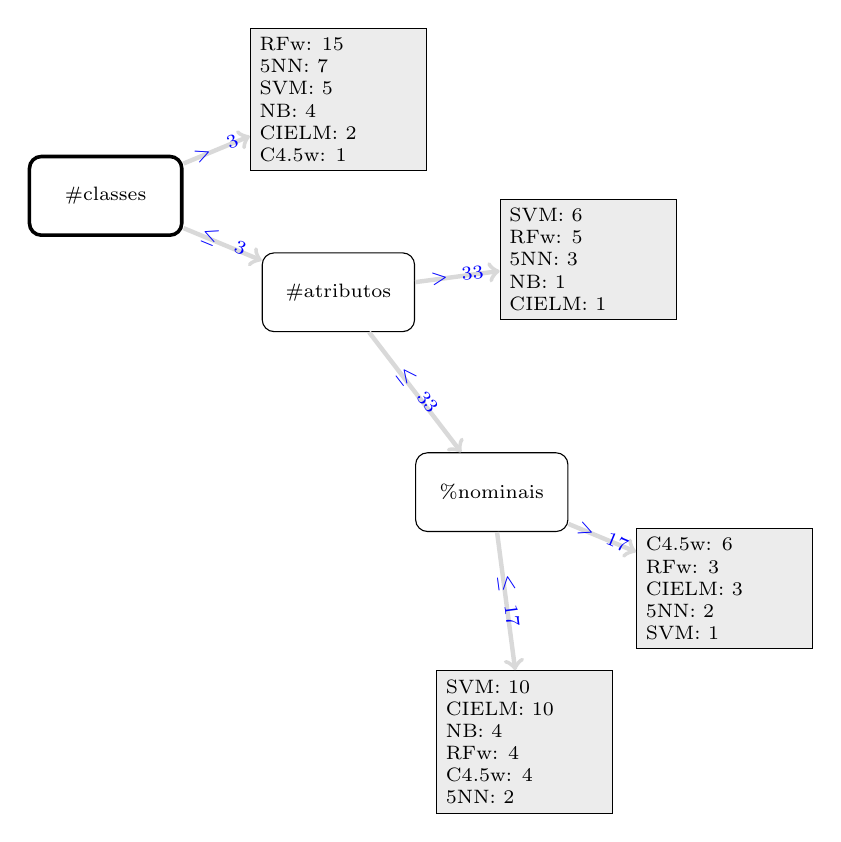
\begin{tikzpicture} [edge from parent/.style={->,above,draw,sloped,midway,gray!30,ultra thick},
text width=2.7cm, align=flush center, grow cyclic,
level 1/.style={level distance=3.2cm,sibling angle=45},
level 2/.style={text width=2cm, font=\footnotesize, level distance=3.2cm,sibling angle=60},
level 3/.style={text width=2cm, font=\footnotesize, level distance=3.2cm,sibling angle=60},
level 4/.style={text width=2cm, font=\footnotesize, level distance=3.2cm,sibling angle=90},
level 5/.style={text width=2cm, font=\footnotesize, level distance=3.2cm,sibling angle=45},
]
\node[line width=0.3ex, decision] {\#classes}
child {node [decision] {\#atributos}
child {node [decision] {\%nominais}
child {node [outcome] {SVM: 10\\
CIELM: 10\\
NB: 4\\
RFw: 4\\
C4.5w: 4\\
5NN: 2} edge from parent node [cond] {$\leq17$}}
child {node [outcome] {C4.5w: 6\\
RFw: 3\\
CIELM: 3\\
5NN: 2\\
SVM: 1} edge from parent node [cond] {$>17$}}edge from parent node [cond] {$\leq33$}}
child {node [outcome] {SVM: 6\\
RFw: 5\\
5NN: 3\\
NB: 1\\
CIELM: 1} edge from parent node [cond] {$>33$}}edge from parent node [cond] {$\leq 3$}}
child {node [outcome] {RFw: 15\\
5NN: 7\\
SVM: 5\\
NB: 4\\
CIELM: 2\\
C4.5w: 1} edge from parent node [cond] {$> 3$}};
\label{treegoodleas}
\end{tikzpicture}
\end{center}
\end{figure}
É possível notar que a distribuição de vitórias muda consideravelmente em cada caminho
possível.
Essa constatação serve de inspiração para o sistema automático de recomendação
de estratégias de aprendizado ativo, no sentido de sugerir a possibilidade de caracterização
de bases sem que os rótulos estejam presentes.


\subsection{Diversidade de estratégias}
É esperado que as estratégias implementadas da literatura e as propostas nesta tese
tenham desempenho heterogêneo no conjunto de bases de dados escolhido.
Para confirmação,
uma árvore com a distribuição de vitórias das estratégias é exposta
na Figura \ref{treeALCKappa}.
Os nomes de estratégias propostas estão em negrito.
Nas análises seguintes, uma abreviação de estratégia seguida de asterisco indica o conjunto
de todas as suas variantes.
\usetikzlibrary{trees}
% \afterpage{\clearpage\begin{landscape}
\begin{figure}
\tikzset{
every node/.style={font=\scriptsize,black, thin},
decision/.style={shape=rectangle, minimum height=1cm, text width=1.7cm,
text centered, rounded corners=1ex, draw},
outcome/.style={ shape=rectangle, fill=gray!15, draw, text width=2cm, text justified},
decision tree/.style={sibling distance=3cm, level distance=2cm},
cond/.style={blue, yshift=-2mm, shape=rectangle, text centered},
}
\begin{center}
\caption{Distribui��o das estrat�gias vencedoras de acordo com o algoritmo usado e
caracter�sticas de cada base.
\textit{As folhas apresentam a frequ�ncia de vit�rias das estrat�gias.
Uma coloca��o entre as tr�s melhores � contabilizada como vit�ria.
As $25\%$ menos frequentes s�o representadas pela categoria ``demais''.
M�nimo de $40$ exemplos por folha.}
}
\begin{tikzpicture} [edge from parent/.style={->,above,draw,sloped,midway,gray!30,ultra thick},
text width=2.7cm, align=flush center, grow cyclic,
level 1/.style={level distance=3.3cm,sibling angle=60},
level 2/.style={text width=2cm, font=\footnotesize, level distance=3.3cm,sibling angle=60},
level 3/.style={text width=2cm, font=\footnotesize, level distance=3.2cm,sibling angle=60},
level 4/.style={text width=2cm, font=\footnotesize, level distance=3.1cm,sibling angle=45},
level 5/.style={text width=2cm, font=\footnotesize, level distance=2.85cm,sibling angle=45},
]
\input treeLearnerfalse
\label{tree1}
\end{tikzpicture}
\end{center}
\end{figure}
\end{landscape}\clearpage}



 a árvore de algs ficou horrivel.
% \begin{center}
\begin{figure}\label{tree}
\caption{�rvore de decis�o gerada pelo algoritmo C4.5 com um m�nimo de $12$ exemplos
por n� (de um total de $188$ pares base-or�amento).
O grau de pureza de cada folha � dado entre par�nteses.
Estrat�gias propostas est�o em negrito.
Rnd, Mar e EERacu n�o tiveram vit�rias suficientes para aparecer na �rvore.
\ano{reposicionar valores para maior proximidade das arestas}}
% \usetikzlibrary{trees}
% \tikzset{
%     every node/.style={        font=\scriptsize    },
%     decision/.style={        shape=rectangle,        minimum height=1cm,
%         text width=1.7cm,        text centered,        rounded corners=1ex,        draw,    },
%     outcome/.style={        shape=ellipse,        fill=gray!15,        draw,
%         text width=1.15cm,        text centered    },
%     decision tree/.style={        sibling distance=3cm,        level distance=2cm    }
% }
\begin{tikzpicture} [text width=2.7cm, align=flush center,grow cyclic,
level 1/.style={level distance=2.5cm,sibling angle=180},
level 2/.style={text width=2cm, font=\footnotesize, level distance=3cm,sibling angle=45}]
\node[line width=0.3ex, decision] {classes}
    child {node [decision, label=$\leq5$] {aprendiz}
      child {node [decision, label=SVM] {$\# atributos$}
        child {node [outcome, label=$\leq7$] {DWeuc ($25\%$)}}
        child {node [outcome, label=$>7$] {\textbf{ATUmah} ($33\%$)}}
      }
      child {node [decision, label=5NN] {or�amento}
        child {node [outcome, label=baixo] {EERent ($40\%$)}}
        child {node [outcome, label=alto] {Mar ($33\%$)}}
      }
      child {node [decision, label=C4.5] {$\frac{|\mathcal{U}|}{\# atributos}$}
        child {node [outcome, label=$\leq50$] {\textbf{ATUeuc} ($22\%$)}}
        child {node [decision, label=$>50$] {or�amento}
          child {node [outcome, label=baixo] {EERent ($33\%$)}}
          child {node [outcome, label=alto] {\textbf{SGmulti} ($25\%$)}}
        }
      }
      child {node [outcome, label=VFDT] {\textbf{ATUeuc} ($32\%$)}}
      child {node [decision, label=NB] {$\# atributos$}
        child {node [outcome, label=$\leq11$] {TUeuc ($25\%$)}}
        child {node [outcome, label=$>11$] {Clu ($36\%$)}}
      }
      child {node [outcome, label=CIELM] {\textbf{TUeuc} ($50\%$)}}
    }
    child {node [decision, label=$>5$] {$\frac{\%maj}{\%min}$}
      child {node [outcome, label=$\leq2$] {\textbf{ATUmah} ($33\%$)}}
      child {node [outcome, label=$>2$] {\textbf{ATUeuc} ($43\%$)}}
    };
\end{tikzpicture}
\end{figure}
\end{center}

\afterpage{\clearpage\begin{landscape}
\begin{figure}
\tikzset{
every node/.style={font=\scriptsize,black, thin},
decision/.style={shape=rectangle, minimum height=1cm, text width=1.7cm,
text centered, rounded corners=1ex, draw},
outcome/.style={ shape=rectangle, fill=gray!15, draw, text width=2cm, text justified},
decision tree/.style={sibling distance=3cm, level distance=2cm},
cond/.style={blue, yshift=-2mm, shape=rectangle, text centered},
}
\begin{center}
\caption{Distribuição das vitórias.
\textit{Uma colocação entre as três melhores é contabilizada como vitória.
% As $25\%$ menos frequentes são representadas pela categoria ``outras''.
}
}
\scalebox{0.9}{
\begin{tikzpicture} [edge from parent/.style={->,above,draw,sloped,midway,gray!30,ultra thick},
text width=2.7cm, align=flush center, grow cyclic,
level 1/.style={level distance=3cm,sibling angle=60},
level 2/.style={text width=2cm, font=\footnotesize, level distance=3.5cm,sibling angle=60},
level 3/.style={text width=2cm, font=\footnotesize, level distance=3.2cm,sibling angle=60},
level 4/.style={text width=2cm, font=\footnotesize, level distance=3.1cm,sibling angle=75},
level 5/.style={text width=2cm, font=\footnotesize, level distance=2.85cm,sibling angle=45},
]
\input treeALCKappa
\label{treeALCKappa}
\end{tikzpicture}
}
\end{center}
\end{figure}
\end{landscape}\clearpage}
% Em cada base, o algoritmo com o pior desempenho passivo foi dispensado
% visando minimizar a ocorrência de testes deficientes,
% pois existem combinações base-algoritmo inadequadas.

Pode-se observar que a estratégia dominante difere conforme o caminho seguido na árvore,
confirmando a expectativa de heterogeneidade.
Outra característica importante é o metaatributo \textit{algoritmo} situar-se como nó raiz,
sugerindo seu papel determinante no sucesso da estratégia e,
consequentemente, a existência de afinidades entre estratégias e algoritmos.

Por outro lado,
também é esperada alguma correlação entre estratégias similares, por exemplo,
entre Ent e Mar na folha posicionada acima do nó raiz.
Similarmente, algumas variantes dos conjuntos ATU*, DW*, HTU*, SVM* e TU*
também têm ocorrências significativas em folhas coincidentes.
% , como:
% \begin{itemize}
%  \item os pares DWeuc-DWmah, EERent-EERacc e SVMsim-SVMbal no caminho\\
% $(algoritmo=NB) \rightarrow (\#classes\leq 4)$;
% \item EERent-EERacc e HTUeuc-HTUman no caminho\\
% $(algoritmo=C4.5w) \rightarrow (\%major.\leq 79)$; ou,
% \item HTUmah-HTUeuc nos caminhos\\ $(algoritmo=5NN)$ e
% $(algoritmo=SVM) \rightarrow (26 < \%major.\leq 78)$.
% \end{itemize}
Assim, há a possibilidade de remoção de estratégias muito similares
visando a facilitação do experimento de análise comparativa,
embora, no experimento posterior de \ano{identificação de nichos de aplicação e de} recomendação
automática, essas estratégias tenham passado a ser \ano{reconsideradas}.

Analogamente à comparação na Seção \ref{algs},
as similaridades entre estratégias foram calculadas
por meio da distância $d(\bm{x},\bm{u}) \mid \bm{x},\bm{u} \in \mathbb{R}^{564}$
entre medidas kappa ao longo das $94$ bases e $6$ algoritmos.
Elas são apresentadas na Tabela \ref{stratDists}.
\afterpage{\clearpage\begin{landscape}
\begin{table}[h]
\caption{Similaridade entre estratégias. Medida: ALC da acurácia balanceada.
\textit{Detalhes na Tabela \ref{passiveDists}.}}
\begin{center}\scalebox{0.77}{
\begin{tabular}{lcc|cc|cc|cc|cc|cc|cc|cc|cc|cc|cc}
                                & \begin{sideways}Rnd\end{sideways} & \begin{sideways}Clu\end{sideways} & \begin{sideways}\textbf{ATUeuc}\end{sideways} & \begin{sideways}\textbf{ATUman}\end{sideways} & \begin{sideways}\textbf{ATUmah}\end{sideways} & \begin{sideways}\textbf{HTUeuc}\end{sideways} & \begin{sideways}\textbf{HTUman}\end{sideways} & \begin{sideways}\textbf{HTUmah}\end{sideways} & \begin{sideways}\textbf{SGmulti}\end{sideways} & \begin{sideways}QBCRFw\end{sideways} & \begin{sideways}Ent\end{sideways} & \begin{sideways}Mar\end{sideways} & \begin{sideways}DWeuc\end{sideways} & \begin{sideways}DWman\end{sideways} & \begin{sideways}DWmah\end{sideways} & \begin{sideways}TUeuc\end{sideways} & \begin{sideways}TUman\end{sideways} & \begin{sideways}TUmah\end{sideways} & \begin{sideways}EERacc\end{sideways} & \begin{sideways}EERent\end{sideways} & \begin{sideways}SVMbal\end{sideways} & \begin{sideways}SVMsim\end{sideways} \\Rnd   & - & \textcolor{blue}{\textbf{  0.64}} & \textbf{  0.58} & \textbf{  0.57} & \textbf{  0.55} &   0.44 &   0.46 &   0.46 & \textbf{  0.57} &   0.37 &   0.37 &   0.37 &   0.25 & \textcolor{red}{\textbf{  0.24}} &   0.26 &   0.40 &   0.40 &   0.41 &   0.46 &   0.38 &   0.33 &   0.30 \\
Clu     & \textcolor{blue}{\textbf{  0.64}} & - & \textbf{  0.57} & \textbf{  0.58} & \textbf{  0.55} &   0.48 & \textbf{  0.50} & \textbf{  0.50} & \textbf{  0.59} &   0.40 &   0.39 &   0.40 &   0.24 & \textcolor{red}{\textbf{  0.23}} &   0.25 &   0.43 &   0.43 &   0.44 & \textbf{  0.51} &   0.41 &   0.34 &   0.30 \\ \hline
\textbf{ATUeuc} & \textbf{  0.58} & \textbf{  0.57} & - & \textcolor{blue}{\textbf{  0.76}} & \textbf{  0.70} &   0.49 & \textbf{  0.51} & \textbf{  0.52} & \textbf{  0.50} &   0.36 &   0.36 &   0.36 &   0.24 & \textcolor{red}{\textbf{  0.23}} &   0.25 &   0.43 &   0.43 &   0.44 &   0.42 &   0.36 &   0.33 &   0.29 \\
\textbf{ATUman} & \textbf{  0.57} & \textbf{  0.58} & \textcolor{blue}{\textbf{  0.76}} & - & \textbf{  0.70} & \textbf{  0.51} & \textbf{  0.54} & \textbf{  0.53} & \textbf{  0.50} &   0.37 &   0.37 &   0.37 &   0.24 & \textcolor{red}{\textbf{  0.23}} &   0.25 &   0.44 &   0.45 &   0.45 &   0.44 &   0.37 &   0.34 &   0.30 \\ \hline
\textbf{ATUmah} & \textbf{  0.55} & \textbf{  0.55} & \textcolor{blue}{\textbf{  0.70}} & \textcolor{blue}{\textbf{  0.70}} & - & \textbf{  0.50} & \textbf{  0.52} & \textbf{  0.54} &   0.48 &   0.36 &   0.36 &   0.36 & \textcolor{red}{\textbf{  0.24}} & \textcolor{red}{\textbf{  0.24}} &   0.25 &   0.43 &   0.44 &   0.45 &   0.43 &   0.36 &   0.33 &   0.30 \\
\textbf{HTUeuc} &   0.44 &   0.48 &   0.49 & \textbf{  0.51} & \textbf{  0.50} & - & \textcolor{blue}{\textbf{  0.71}} & \textbf{  0.64} &   0.47 &   0.38 &   0.42 &   0.43 &   0.25 & \textcolor{red}{\textbf{  0.24}} &   0.26 & \textbf{  0.58} & \textbf{  0.60} & \textbf{  0.60} &   0.45 &   0.38 &   0.33 &   0.29 \\ \hline
\textbf{HTUman} &   0.46 & \textbf{  0.50} & \textbf{  0.51} & \textbf{  0.54} & \textbf{  0.52} & \textcolor{blue}{\textbf{  0.71}} & - & \textbf{  0.66} &   0.49 &   0.39 &   0.41 &   0.42 &   0.24 & \textcolor{red}{\textbf{  0.23}} &   0.25 & \textbf{  0.52} & \textbf{  0.55} & \textbf{  0.54} &   0.47 &   0.39 &   0.33 &   0.29 \\
\textbf{HTUmah} &   0.46 & \textbf{  0.50} & \textbf{  0.52} & \textbf{  0.53} & \textbf{  0.54} & \textbf{  0.64} & \textcolor{blue}{\textbf{  0.66}} & - &   0.48 &   0.38 &   0.40 &   0.41 &   0.24 & \textcolor{red}{\textbf{  0.23}} &   0.25 & \textbf{  0.51} & \textbf{  0.53} & \textbf{  0.55} &   0.45 &   0.38 &   0.33 &   0.29 \\ \hline
\textbf{SGmulti}        & \textbf{  0.57} & \textcolor{blue}{\textbf{  0.59}} & \textbf{  0.50} & \textbf{  0.50} &   0.48 &   0.47 &   0.49 &   0.48 & - &   0.37 &   0.41 &   0.42 &   0.24 & \textcolor{red}{\textbf{  0.23}} &   0.25 &   0.42 &   0.43 &   0.43 & \textbf{  0.51} &   0.39 &   0.32 &   0.28 \\
QBCRFw  &   0.37 & \textcolor{blue}{\textbf{  0.40}} &   0.36 &   0.37 &   0.36 &   0.38 &   0.39 &   0.38 &   0.37 & - &   0.36 &   0.35 &   0.25 & \textcolor{red}{\textbf{  0.24}} &   0.25 &   0.37 &   0.38 &   0.37 &   0.38 &   0.36 &   0.37 &   0.33 \\ \hline
Ent     &   0.37 &   0.39 &   0.36 &   0.37 &   0.36 &   0.42 &   0.41 &   0.40 &   0.41 &   0.36 & - & \textcolor{blue}{\textbf{  0.62}} & \textcolor{red}{\textbf{  0.24}} & \textcolor{red}{\textbf{  0.24}} &   0.25 &   0.47 &   0.47 &   0.45 &   0.42 &   0.35 &   0.31 &   0.28 \\
Mar     &   0.37 &   0.40 &   0.36 &   0.37 &   0.36 &   0.43 &   0.42 &   0.41 &   0.42 &   0.35 & \textcolor{blue}{\textbf{  0.62}} & - &   0.24 & \textcolor{red}{\textbf{  0.23}} &   0.25 & \textbf{  0.50} &   0.49 &   0.47 &   0.45 &   0.36 &   0.30 &   0.27 \\ \hline
DWeuc   &   0.25 &   0.24 &   0.24 &   0.24 &   0.24 &   0.25 &   0.24 &   0.24 &   0.24 &   0.25 &   0.24 &   0.24 & - & \textcolor{blue}{\textbf{  0.52}} &   0.40 &   0.25 &   0.25 &   0.25 &   0.24 & \textcolor{red}{\textbf{  0.22}} &   0.26 &   0.25 \\
DWman   &   0.24 &   0.23 &   0.23 &   0.23 &   0.24 &   0.24 &   0.23 &   0.23 &   0.23 &   0.24 &   0.24 &   0.23 & \textcolor{blue}{\textbf{  0.52}} & - &   0.42 &   0.24 &   0.24 &   0.24 &   0.23 & \textcolor{red}{\textbf{  0.22}} &   0.25 &   0.25 \\ \hline
DWmah   &   0.26 &   0.25 &   0.25 &   0.25 &   0.25 &   0.26 &   0.25 &   0.25 &   0.25 &   0.25 &   0.25 &   0.25 &   0.40 & \textcolor{blue}{\textbf{  0.42}} & - &   0.26 &   0.25 &   0.26 &   0.25 & \textcolor{red}{\textbf{  0.23}} &   0.25 &   0.25 \\
TUeuc   &   0.40 &   0.43 &   0.43 &   0.44 &   0.43 & \textbf{  0.58} & \textbf{  0.52} & \textbf{  0.51} &   0.42 &   0.37 &   0.47 & \textbf{  0.50} &   0.25 & \textcolor{red}{\textbf{  0.24}} &   0.26 & - & \textcolor{blue}{\textbf{  0.74}} & \textbf{  0.64} &   0.43 &   0.35 &   0.32 &   0.29 \\ \hline
TUman   &   0.40 &   0.43 &   0.43 &   0.45 &   0.44 & \textbf{  0.60} & \textbf{  0.55} & \textbf{  0.53} &   0.43 &   0.38 &   0.47 &   0.49 &   0.25 & \textcolor{red}{\textbf{  0.24}} &   0.25 & \textcolor{blue}{\textbf{  0.74}} & - & \textbf{  0.66} &   0.43 &   0.36 &   0.32 &   0.29 \\
TUmah   &   0.41 &   0.44 &   0.44 &   0.45 &   0.45 & \textbf{  0.60} & \textbf{  0.54} & \textbf{  0.55} &   0.43 &   0.37 &   0.45 &   0.47 &   0.25 & \textcolor{red}{\textbf{  0.24}} &   0.26 & \textbf{  0.64} & \textcolor{blue}{\textbf{  0.66}} & - &   0.42 &   0.36 &   0.32 &   0.28 \\ \hline
EERacc  &   0.46 & \textcolor{blue}{\textbf{  0.51}} &   0.42 &   0.44 &   0.43 &   0.45 &   0.47 &   0.45 & \textcolor{blue}{\textbf{  0.51}} &   0.38 &   0.42 &   0.45 &   0.24 & \textcolor{red}{\textbf{  0.23}} &   0.25 &   0.43 &   0.43 &   0.42 & - &   0.44 &   0.33 &   0.30 \\
EERent  &   0.38 &   0.41 &   0.36 &   0.37 &   0.36 &   0.38 &   0.39 &   0.38 &   0.39 &   0.36 &   0.35 &   0.36 & \textcolor{red}{\textbf{  0.22}} & \textcolor{red}{\textbf{  0.22}} &   0.23 &   0.35 &   0.36 &   0.36 & \textcolor{blue}{\textbf{  0.44}} & - &   0.30 &   0.27 \\ \hline
SVMbal  &   0.33 &   0.34 &   0.33 &   0.34 &   0.33 &   0.33 &   0.33 &   0.33 &   0.32 &   0.37 &   0.31 &   0.30 &   0.26 & \textcolor{red}{\textbf{  0.25}} & \textcolor{red}{\textbf{  0.25}} &   0.32 &   0.32 &   0.32 &   0.33 &   0.30 & - & \textcolor{blue}{\textbf{  0.54}} \\
SVMsim  &   0.30 &   0.30 &   0.29 &   0.30 &   0.30 &   0.29 &   0.29 &   0.29 &   0.28 &   0.33 &   0.28 &   0.27 & \textcolor{red}{\textbf{  0.25}} & \textcolor{red}{\textbf{  0.25}} & \textcolor{red}{\textbf{  0.25}} &   0.29 &   0.29 &   0.28 &   0.30 &   0.27 & \textcolor{blue}{\textbf{  0.54}} & - \\ \hline\end{tabular}
}
\label{stratDists}
\end{center}
\end{table}
\end{landscape}\clearpage}
As estratégias mais exploratórias (Rnd, Clu, ATU* e SGmulti)
tiveram entre si um grau de similaridade acima da média
(valor de $0,64$ para as duas primeiras e entre $0,48$ e $0,50$ para as restantes,
desconsiderando variantes da mesma estratégia entre si).
Entretanto, Rnd, Clu e SGmulti foram mantidas pelo seu valor referencial e histórico.
Uma similaridade maior pode ser notada dentro dos três conjuntos de variantes
ATU*, HTU* e TU* (entre $0,64$ e $0,76$), logo,
é possível manter apenas uma das métricas de distância sem impactar
significativamente a representatividade das estratégias.
Assim, as variantes baseadas nas distâncias euclidiana e de Manhattan
foram excluídas por serem mais similares às demais variantes do que as baseadas na
distância de Mahalanobis de acordo com a Tabela \ref{stratDists}:
\begin{itemize}
\item TUeuc: $0,74$ e $0,64$, TUman: $0,74$ e $0,66$, \textbf{TUmah}: $0,66$ e $0,64$;
\item ATUeuc: $0,76$ e $0,70$, ATUman: $0,76$ e $0,70$, \textbf{ATUmah}: $0,70$ e $0,70$;
\item HTUeuc: $0,71$ e $0,64$, e HTUman: $0,71$ e $0,66$, \textbf{HTUmah}: $0,64$ e $0,66$,
 \end{itemize}
Além disso, a intrínseca independência de escala da distância de Mahalanobis é uma
característica que teoricamente a torna menos vinculada ao formato dos atributos.

Dentre as estratégias baseadas em simples medida de informatividade
(Unc, Ent e Mar), apenas Mar foi mantida devido
à sua considerável similaridade com Ent ($0,62$),
por ser equivalente em problemas binários e mais adequada a problemas multiclasse que Unc
e por seu desempenho superior\footnote{\label{note1}Detalhes nas tabelas
\ref{strats0a5NN}, \ref{strats1a5NN}, \ref{strats2a5NN},
\ref{strats0b5NN}, \ref{strats1b5NN}, \ref{strats2b5NN},
\ref{strats0aC4.5w}, \ref{strats1aC4.5w}, \ref{strats2aC4.5w},
\ref{strats0bC4.5w}, \ref{strats1bC4.5w}, \ref{strats2bC4.5w},
\ref{strats0aNB}, \ref{strats1aNB}, \ref{strats2aNB},
\ref{strats0bNB}, \ref{strats1bNB}, \ref{strats2bNB},
\ref{strats0aCIELM}, \ref{strats1aCIELM}, \ref{strats2aCIELM},
\ref{strats0bCIELM}, \ref{strats1bCIELM}, \ref{strats2bCIELM},
\ref{strats0aRFw}, \ref{strats1aRFw}, \ref{strats2aRFw},
\ref{strats0bRFw}, \ref{strats1bRFw}, \ref{strats2bRFw},
\ref{strats0aSVM}, \ref{strats1aSVM}, \ref{strats2aSVM},
\ref{strats0bSVM}, \ref{strats1bSVM} e \ref{strats2bSVM}
do Apêndice \ref{detalhes}.}.
As variantes DW* são as mais dissimilares (entre $0,22$ e $0,26$) devido a seu desempenho
geral excessivamente inferior\footref{note1}.
Por esse motivo, e principalmente por serem melhor representadas pelas suas sucessoras TU*,
nenhuma delas foi mantida.
% Analogamente à escolha feita com as outras estratégias baseadas em distância,
% apenas a de Mahalanobis foi mantida.
Finalmente,
SVMbal foi mantida em detrimento de SVMsim, por ser similar, sua sucessora e ter
um desempenho melhor\footref{note1}; e,
EERacc foi eliminada por ser inferior a EERent, pois
a acurácia como função objetivo não foi bem sucedida quando comparada à medida
de entropia - função utilizada no trabalho original\footref{note1}.
\ano{descrever no apêndice como fazer pra descobrir essas conclusões das tabelas,
talvez com friedman}
O grupo reduzido de dez estratégias é apresentado na Tabela \ref{stratDistsRedux}.
\begin{table}[h]
\caption{Similaridade entre estratégias selecionadas.  Medida: ALC da acurácia balanceada.
\textit{Detalhes na Tabela \ref{passiveDists}.}}
\begin{center}
\scalebox{0.94}{
\begin{tabular}{lcc|cc|cc|cc|cc}
 & Rnd & Clu & \textbf{\makecell{ATU\\mah}} & \textbf{\makecell{HTU\\mah}} & \textbf{\makecell{SG\\multi}} & QBC & Mar & \makecell{TU\\mah} & \makecell{EER\\ent} & \makecell{SVM\\bal} \\
 \hline
  Rnd       & - & \textcolor{blue}{\textbf{  0.64}} & \textbf{  0.55} &   0.46 & \textbf{  0.57} &   0.37 &   0.37 &   0.41 &   0.38 & \textcolor{red}{\textbf{  0.33}} \\
Clu     & \textcolor{blue}{\textbf{  0.64}} & - & \textbf{  0.55} & \textbf{  0.50} & \textbf{  0.59} &   0.40 &   0.40 &   0.44 &   0.41 & \textcolor{red}{\textbf{  0.34}} \\ \hline
\textbf{ATUmah} & \textcolor{blue}{\textbf{  0.55}} & \textcolor{blue}{\textbf{  0.55}} & - & \textbf{  0.54} &   0.48 &   0.36 &   0.36 &   0.45 &   0.36 & \textcolor{red}{\textbf{  0.33}} \\
\textbf{HTUmah} &   0.46 & \textbf{  0.50} & \textbf{  0.54} & - &   0.48 &   0.38 &   0.41 & \textcolor{blue}{\textbf{  0.55}} &   0.38 & \textcolor{red}{\textbf{  0.33}} \\ \hline
\textbf{SGmulti}        & \textbf{  0.57} & \textcolor{blue}{\textbf{  0.59}} &   0.48 &   0.48 & - &   0.37 &   0.42 &   0.43 &   0.39 & \textcolor{red}{\textbf{  0.32}} \\
QBCRFw  &   0.37 & \textcolor{blue}{\textbf{  0.40}} &   0.36 &   0.38 &   0.37 & - & \textcolor{red}{\textbf{  0.35}} &   0.37 &   0.36 &   0.37 \\ \hline
Mar     &   0.37 &   0.40 &   0.36 &   0.41 &   0.42 &   0.35 & - & \textcolor{blue}{\textbf{  0.47}} &   0.36 & \textcolor{red}{\textbf{  0.30}} \\
TUmah   &   0.41 &   0.44 &   0.45 & \textcolor{blue}{\textbf{  0.55}} &   0.43 &   0.37 &   0.47 & - &   0.36 & \textcolor{red}{\textbf{  0.32}} \\ \hline
EERent  &   0.38 & \textcolor{blue}{\textbf{  0.41}} &   0.36 &   0.38 &   0.39 &   0.36 &   0.36 &   0.36 & - & \textcolor{red}{\textbf{  0.30}} \\
SVMbal  &   0.33 &   0.34 &   0.33 &   0.33 &   0.32 & \textcolor{blue}{\textbf{  0.37}} & \textcolor{red}{\textbf{  0.30}} &   0.32 & \textcolor{red}{\textbf{  0.30}} & - \\ \hline\end{tabular}
\label{stratDistsRedux}
}
\end{center}
\end{table}
Note-se que os critérios adotados na eliminação de abordagens não se configuram como
sobre ajustamento aos conjuntos de dados, pois apesar de serem coincidentemente inferiores,
as eliminadas foram preteridas em favor das alternativas mais adequadas:
implementação usual (EERent), sucessoras (TU* e SVMbal) e
mais genéricas (distância de Mahalanobis).

%%%%%%%%%%%%%%%%%%%%%%%%%%%%%%%
\input exp-analise


não é do conhecimento do autor a existência de trabalhos que empreguem a medida de distância
de Mahalanobis.